\documentclass{article}
\usepackage[utf8]{inputenc}
\usepackage{graphicx}

\title{Language Technology Practical}
\author{Thijs Eker, Niels Visscher, Kenneth Muller, Maaike Los }
\date{June 2017}

\begin{document}

\maketitle

\section{Introduction}

The goal of the assignment was to create a system that answers questions in natural language and queries an open linked data source (in this case, Wikidata) in order to find the answers to those questions. We were to use Python3 for development and Sparql for querying the Wikidata database.

\section{How the system works}
Instead of creating one system that can deal with all questions, we decided to work out three different subsystems that all try to answer the questions, and combine their answers. Because the three systems are essentially different in the way they retrieve their answers, we hope to have an increased probability to be able to answer many different types of questions. \\
After having all three systems run over a question, we checked whether or not there were two or more systems that gave the same answer. If this is the case, this became our final answer. Otherwise, we looked at respectively system 1, system 2 and system 3 in this order whether they found and answer and return that answer. We chose this order because in our test sessions (on the student made question file), system 1 had the highest percentage of correct answers and system 3 the lowest.
Now we will describe the individual systems in more depth:

\section*{System 1}
The main idea behind our first system is that it analyzes the 1025 question-answer pairs provided on Nestor and learns which parts of the sentence should be queried to get the correct answer.
\subsection*{Creating a key}
To figure out which sentences should be treated the same, the system does not look at the words in the sentence, but only to the dependencies. When the system gets a question like 'Which food maker has the most employees?'. We choose to first translate the sentence to a key. In this case the key would look like: \textit{ROOTnsubjdetcompounddobjdetamodpunct}(just the dependencies in the order of the three). This approach makes the system recognize some sentences that are the same, but not enough. To make the keys more general we left out a lot of dependencies. Things like det, punct and other dependencies that say less about the sentence. Furthermore we also concatenate the compound nouns and adjetives(conjunctions are also concatenated). After this the key we end up with is \textit{ROOTnsubjdobj}, which is general enough. Figure .. shows how we change the dependency tree to get the correct key. 
\begin{figure}[!ht]
    \centering
        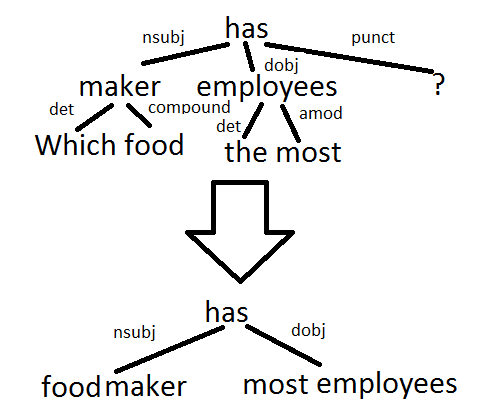
\includegraphics[width=7cm]{secondtree}
    \caption{Original dependency tree and adjusted tree}
    \label{fig:afb5}
\end{figure}

\subsection*{X of Y questions}
Now that we have one key for a lot of similar sentences the process is already a bit easier. For every key we keep two small arrays, that indicate which nouns and verbs are good candidates as entity and which are good as a property. If the entity array has the highest value for the first noun, this means that it most likely is the entity we want to use. And if the property array has a high value for the second noun this probably is the property we need to use.\\
To learn how to solve X of Y questions we simply take all the nouns and verbs from the sentence and try to combine them in a query(one as property and one as entity). For the sentence 'Who founded Burger King', this would be 'Burger king' as property and 'founded' as entity'. After we check the answer we add 1 to the second place of the entity array(the second noun was the correct entity) and also add 1 to the first place of the property array to indicate that the second noun was the property.\\
When we later have to answer X of Y questions we translate the sentence to a key and simply look which nouns or verbs had good results in similar sentences(according to the 2 arrays).

\subsection*{Other questions}
We also analyzed the questions file to see which keys normally describe boolean or 'What is' questions. When we encounter such a key we solve these questions in a normal way, which is not to hard. For boolean questions we just query all combinations of the nouns in the sentence. First with a free property and two given entities. This works for questions like 'Does chocolate contain sugar?', because one of the queries will be something like \textbf{ASK(\{chocolate ?prop sugar\}}. For questions like 'Does soylent have a official site?' we also try queries like \textbf{ASK\{soylent officialSite ?enitity\}}.\\
In the case of a what is question we just ask for a description.

\section*{System 2}

At the base of this system is a construction that answers "the X of Y" in the following form: A list of entities and properties is given, in which one element in the list is the property of the next element of the list. For example, "the mother of the queen of England" is parsed and stored as $["mother", "queen", "England"]$. Upon evaluation, the queen of England is looked up, after which the outcome is used to find the mother of the retrieved person. No maximum length of this list structure is defined, and multiple answers may be found, which are all used in the next iteration, until the list is empty.\\

The interpretation of questions is based upon regular expressions in Python, by extracting relevant information in this array format, and evaluating it afterwards. Different regex patterns were defined to be able to handle as many different questions as possible.\\

The following types of questions were supported:\\

\begin{itemize}
	\item Generic `What is' questions.
	\item `Who did' questions, like `Who founded Burger King?'
	\item Imperatives, e.g. `List the ingredients of a pizza'
	\item Counting questions, e.g. `How many households does Emmen have?'
	\item `Named after' questions, like `What person was Earl Grey Tea named after?'
\end{itemize}

NLP processing with Spacy was used in some cases, however the system was not made to depend on it too much, as its output appeared slightly unreliable in test runs. Instead, it was used to find lemma forms of words in the input (mainly to make sure the queries contained singular forms instead of plural forms) and to verify that (in the `Who did' and `Imperaties' cases) a word was verb.\\

Counting was done in three different ways. The requested property could be availeble as a number (employees of McDonald's, for example), in which cases the output could be used directly. In a second case, there might be a property called `Number of X', for example in `Number of households'. In the third case, every `X' was stored independently (like the ingredients in bread), and the program had to count them. All these possibilities were tried, and in case more than one of them yielded an answer (for example, `employees' of `McDonald's' returned an answer, but the number of fields could be counted as well) the highest number was returned as an answer.\\

The `Who did' were given special attention as well; In the example question `Who founded Burger King?', we would like to find the `founder' of `Burger King', so after verifying that the second word was indeed a verb, the system tried to convert this verb into the `agent' carrying out the action, by again making minimal use of Spacy to find the lemma form, and trying to find it in a specified list of known agents. If it could not be found, it would try to form the agent by appending an `r' if the lemma ended with an `e', and `er' otherwise, which appears to work for English quite often.\\

\section*{System 3}

This system determines what type of question is being asked based on either NLP dependencies or the first word of the sentence. It is capable of distinguishing between four types of questions.\\
First of all, boolean questions, which are questions where either yes or no is the expected answer. These questions can be identified by having a sentence that starts with one of the following verbs: 'be', 'do', 'can' or 'have' (e.g. Is white the color of milk?). We solve these questions by extracting the two entities from the sentence and putting these into an ask query which has the following form:\\
'ASK{ entity1 ?free entity2}'. This will result in a boolean answer which we convert to yes or no.\\
Secondly, we have answers which ask for a location. Location-based questions are identified when a given sentence start with the word 'where' (e.g. Where are the headquarters of the KFC?). The way this was handled was by taking 'location' as the property and then extracting the entity from the question.\\
Thirdly, there are description questions. Description questions are generally structured like 'Who/what is x?', which requires us to search for the wikidata description of the given x (e.g. What is a tomato?). Similarly to how names instead of Q-values are obtained by asking for a label in SPARQL, we can also obtain the description of a given entity in a SPARQL query by adding ?entityDescription to the SELECT statement.\\
Finally, we have the 'x of y' questions, which are generally sentences which provide us with an entity to search for (y) and the property of this entity (x) (e.g. What is the country of origin of spaghetti?).\\
To find the properties and/or entities, we used the NLP dependencies which were obtained through the use of spaCy. These values are different for each of the question types, and they may differ within these types. The dependencies that we used to obtain our properties and entities are based on the questions which can be found on the nestor page. Furthermore, we needed to be able to properly obtain compounds. To do this, for every entity or property that we found, we looked into the subtree provided by spaCy and checked if any of the words in this subtree had a dependency of 'compound' or 'amod'. If this is the case then this should be added to the given entity or property, otherwise it should not.\\
After we have obtained these entities and properties, we have to obtain proper values to send into our SPARQL queries. Originally we were given the choice between an API or anchortexts, but we decided to combine both methods. We compile a list with the top-5 results, such that we end up with a list of at most 10 results, from both the API and the anchortexts. These results are then one-by-one used for our SPARQL query until we obtain an answer. If we cannot obtain an answer after looping through the entire list, we return an empty list.\\

\subsection*{Evaluation}
To get a good feel of how our system performed we continuously ran our system on the 1025 questions(mostly looking at recall). In the beginning our system would only try to solve X of Y questions in the most basic ways and we had score of around 350 questions answered. After refining the three systems and adding functionality for what is, yes/no and count questions we doubled that score.
\subsection*{Test questions}
On the test set of 50 questions, we gave 29 correct answers of 35 answers in total. The most important weakness of our system were questions like 'Which company produces frappucino?' or 'List products which contain goat milk.'. In these question we need to search for certain entity that has a property that is given. This would result in a query like \textbf{SELECT \{?entity contains milk\}}. None of the three systems had the possibility for queries like this. Since we only rarely encountered these kind of questions in the student made question file, we must have overlooked the potential of adding functionality for these questions.\\
One of the better points of our system solving yes/no questions: out of the 6 boolean questions we answered 5 correct.

\section*{Accountability}
Together we attended a few lab sessions and sketched out our plan. The python script calling the answer-question functions from the individual script was also written as a group. The report was also written as a group. For the different systems we had a more individual approach with Thijs working on system one, Niels working on system two and Maaike and Kenneth working on system three.

\end{document}